\section{Portal by Example}
\label{sec:example}

\begin{figure}
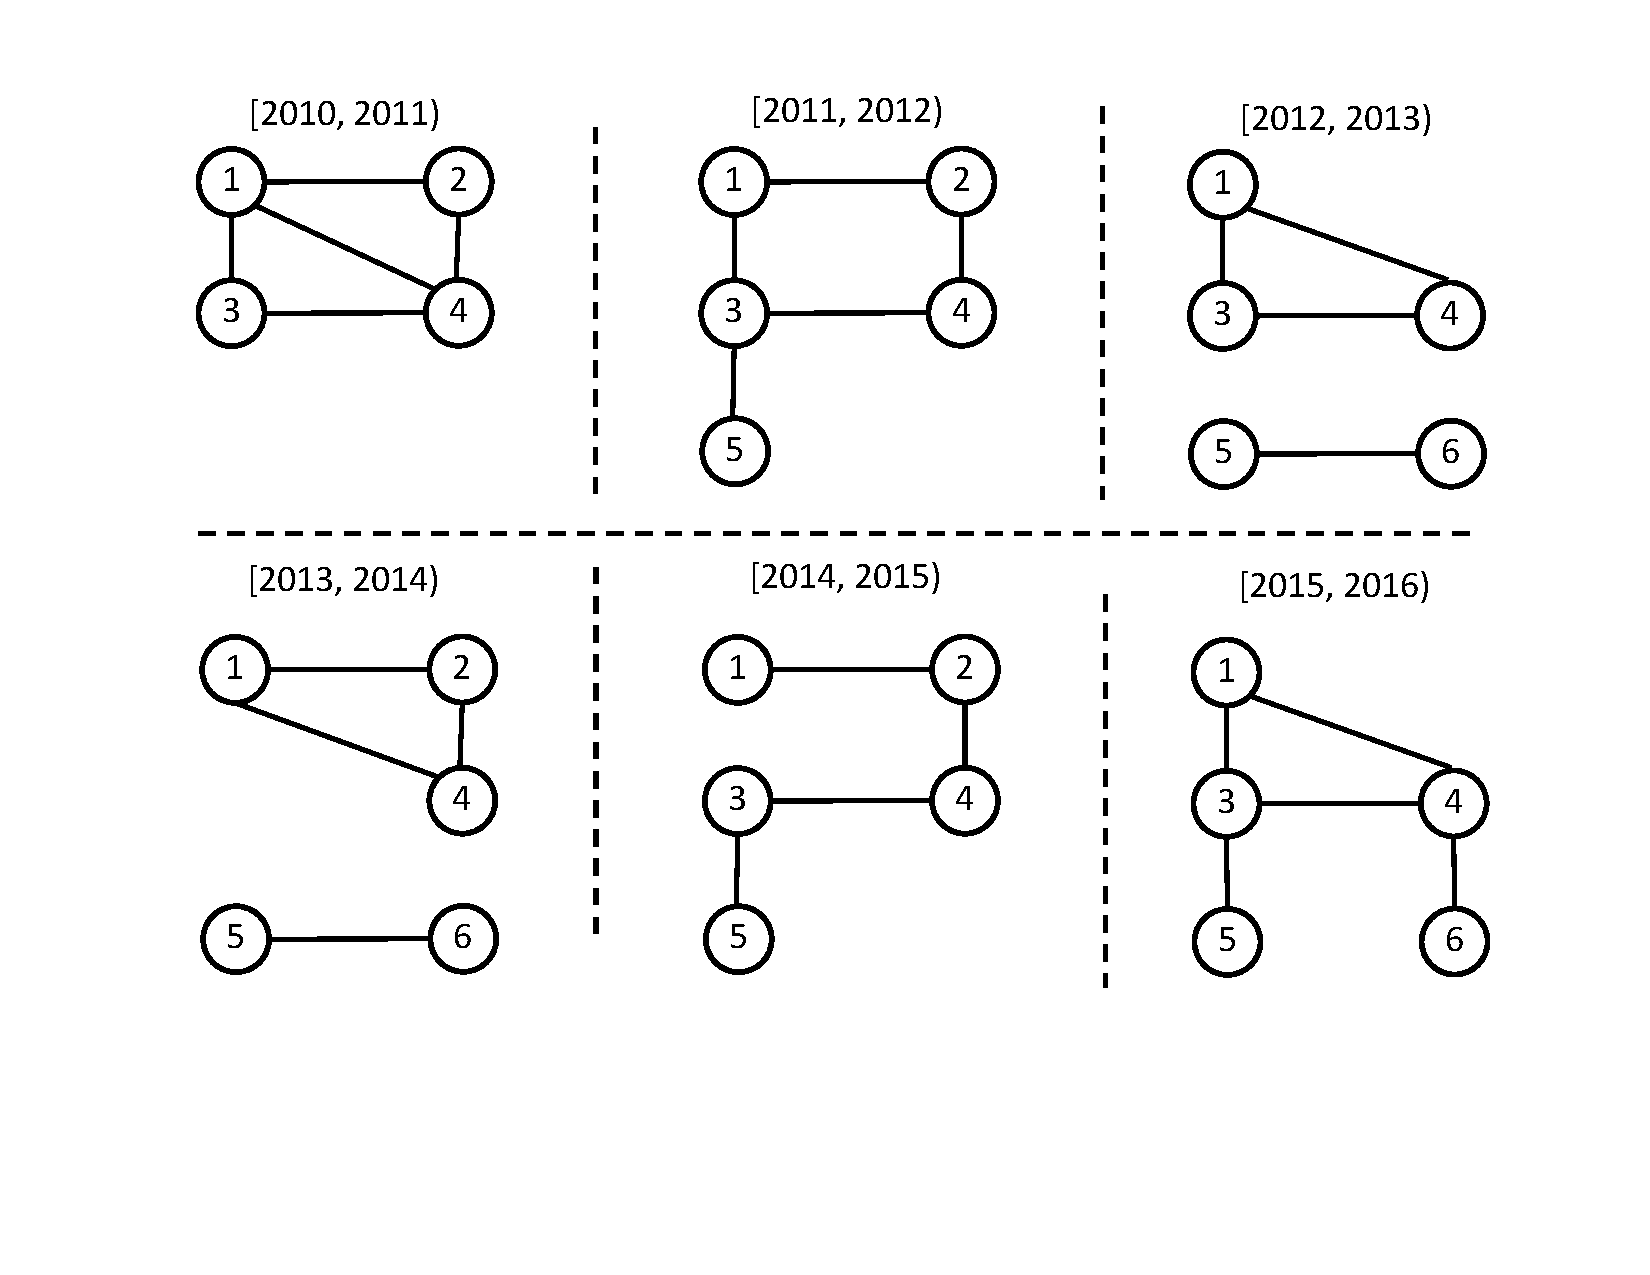
\includegraphics[width=3.2in]{figs/6snaps.pdf}
\caption{A \tg with 6 snapshots.} 
\label{fig:tg}
\end{figure}

In this section we illustrate the salient features of \ql, a
declarative query language for evolving graphs.  A \ql query is
rewritten into a sequence of algebraic operators, a particular
execution method is selected for each operator, and the query is
executed.  All language operators are also available through the
public API of the \ql library, and may be used like any other library
in an Apache Spark application.  We will discuss how \ql queries are
evaluated in Section~\ref{sec:sys}.

Suppose that \tt{T} is the \tg of Figure~\ref{fig:tg}, with the
structural schema V(\underline{vid}:int, name:str, salary:int);
E(\underine{vid1}:int, \underline{vid2}:int, cnt: int).

Query Q1 performs {\em temporal selection} --- it computes a new \tg
\tt{T1} that contains a consecutive subset of the snapshots of \tt{T},
and has the same structural schema as \tt{T}.  Note that the \tt{Into}
clause is optional.

\begin{verbatim}
Q1:   TSelect  V; E
      From     T
      Into     T1
      Start    2010 End 2014
\end{verbatim}

The \tt{TSelect} clause allows us to modify the structural schema of
the result.  We may use this clause to project out non-key columns of
\tt{V} and \tt{E}, or to add columns with computed values.  Consider
query Q2, which computes \tt{T2} from \tt{T}, with vertex schema
V(\underline{vid}:int, name:str, bonus:float, pr:float) and edge
schema E(\underine{vid1}:int, \underline{vid2}:int).  Data types of
computed attributes \tt{bonus} and \tt{pr} are determined by the
return type of the expression that computes them.  Note that \tt{pr}
is computed using the analytic function \tt{pagerank()}.

\begin{verbatim}
Q2:   TSelect  V [vid, name, sal * 0.05 as bonus, pagerank() as pr]; 
               E [vid1, vid2]
      From     T
      Into     T2
\end{verbatim}

The next feature of \ql is temporal aggregation, illustrated by query
Q3, which, when executed on \tt{T} from Figure~\{fig:tg} computes
  \tt{T3} in Figure~\ref{fig:tg_any}.  Temporal aggregation maps one
  or several consecutive snapshots from the input \tg to a single
  snapshot in the output.  How many input snapshots are mapped to one
  snapshot in the output is specified in the \tt{TGroup} clause.  Note
  the use of modifiers \tt{Any} in the \tt{TSelect} clause.  This
  modifier specifies that the output contains a union of the vertices
  (resp. edges) from the snapshots being aggregated.  In our example,
  the snapshot $[2010, 2012)$ in \tt{T3} is computed from snapshots
    $[2010, 2011)$ and $[2011, 2012)$ in \tt{T} and contains 5
        vertices and 6 edges.

\begin{verbatim}
Q3:  TSelect   Any V ; Any E 
     From      T
     Into      T3
     TGroup    by 2 years
\end{verbatim}

\begin{figure}
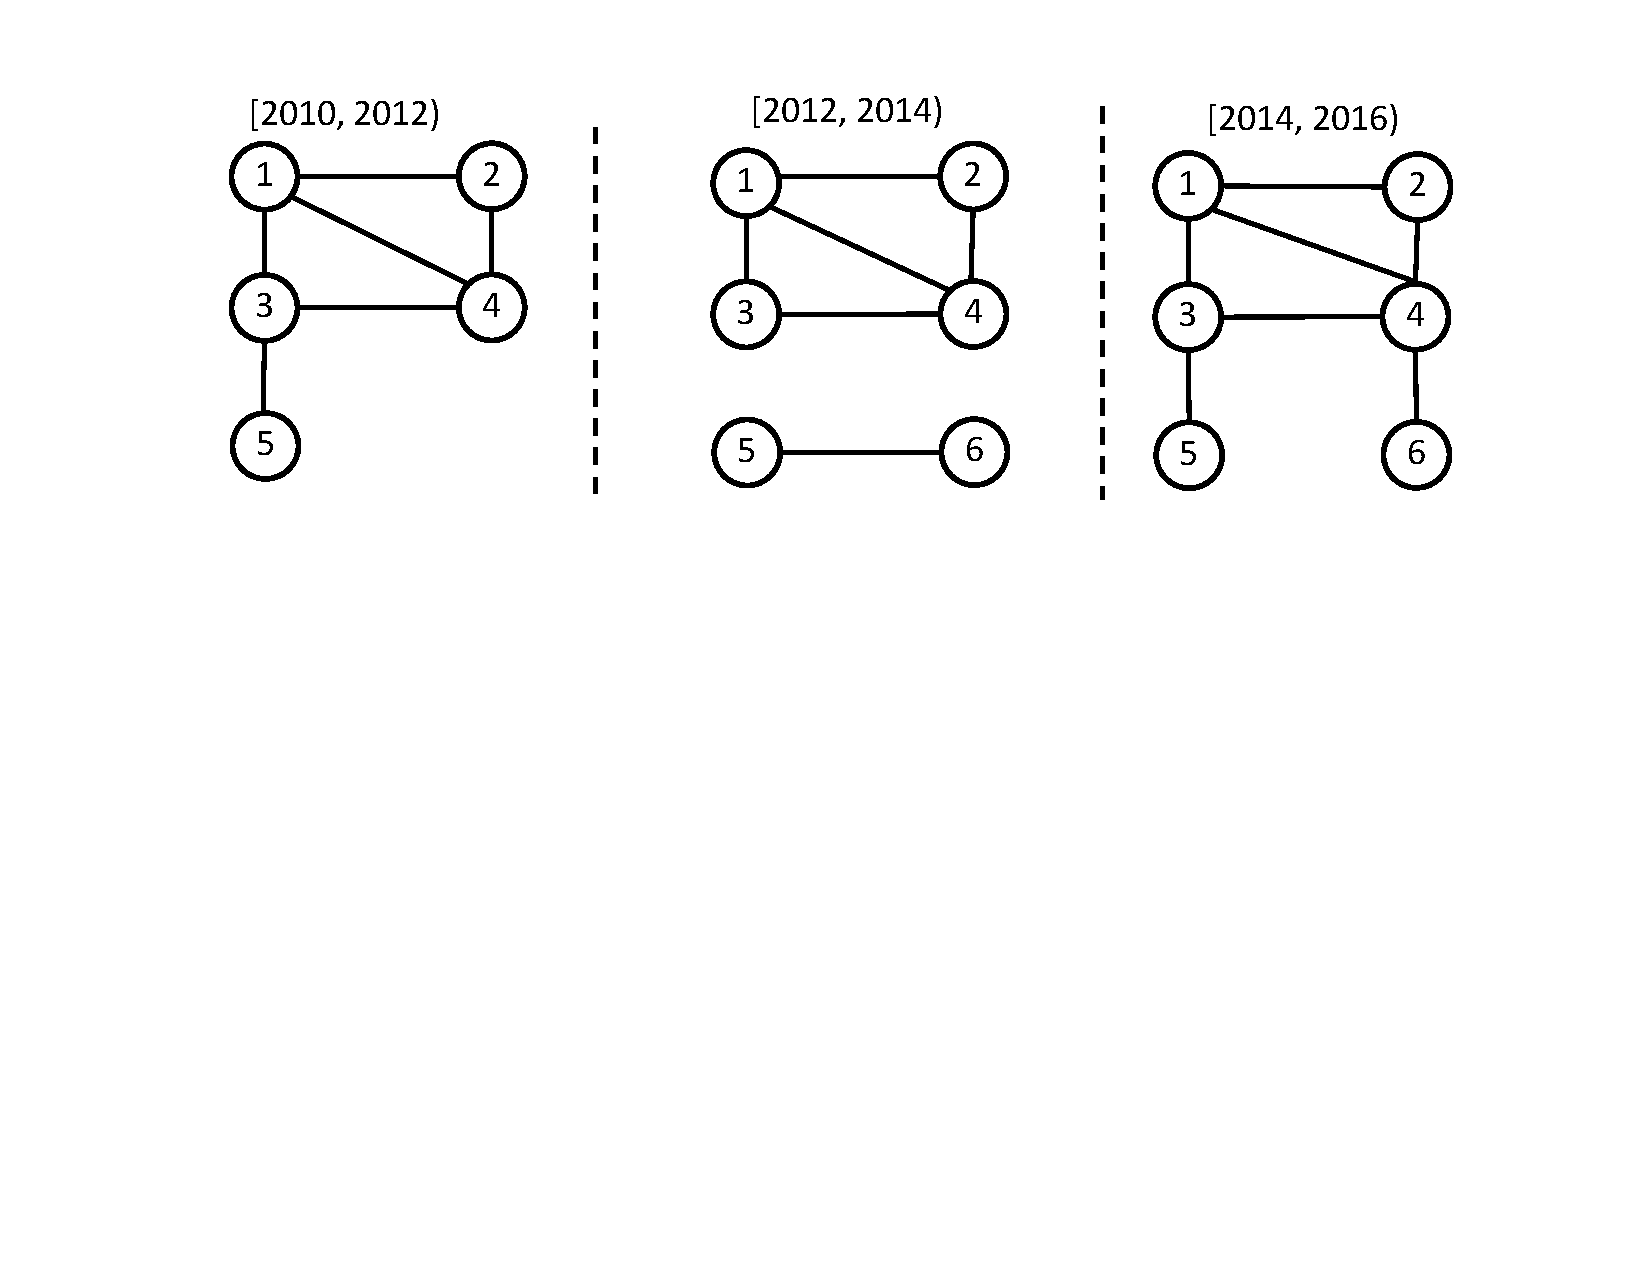
\includegraphics[width=3.2in]{figs/TGroupAny.pdf}
\caption{Result of query Q3.}
\label{fig:tg_any}
\end{figure}

Consider next query Q4, which differs from Q3 only in the use of
\tt{All} modifier associated with edges in the \tt{TSelect} clause.
The result of this query is presented in Figure~\ref{tg_all}.  The
edges in snapshots of \tt{T3} correspond to edges in the intersection
of the snapshots from \tt{T} being aggregated.  As our example
illustrates, \tt{Any} and \tt{All} modifiers can be associated with
vertices or edges or both, and are orthogonal, subject to the
constraint that an edge can only be present in a snapshot if both
vertices it connects are present.

\begin{verbatim}
Q4:   TSelect All V [vid, any(name), max(salary)] ; Any E [vid1, vid2, sum(cnt)] 
      From T 
      Into T4 
      TGroup by 2 years
\end{verbatim}

\begin{figure}
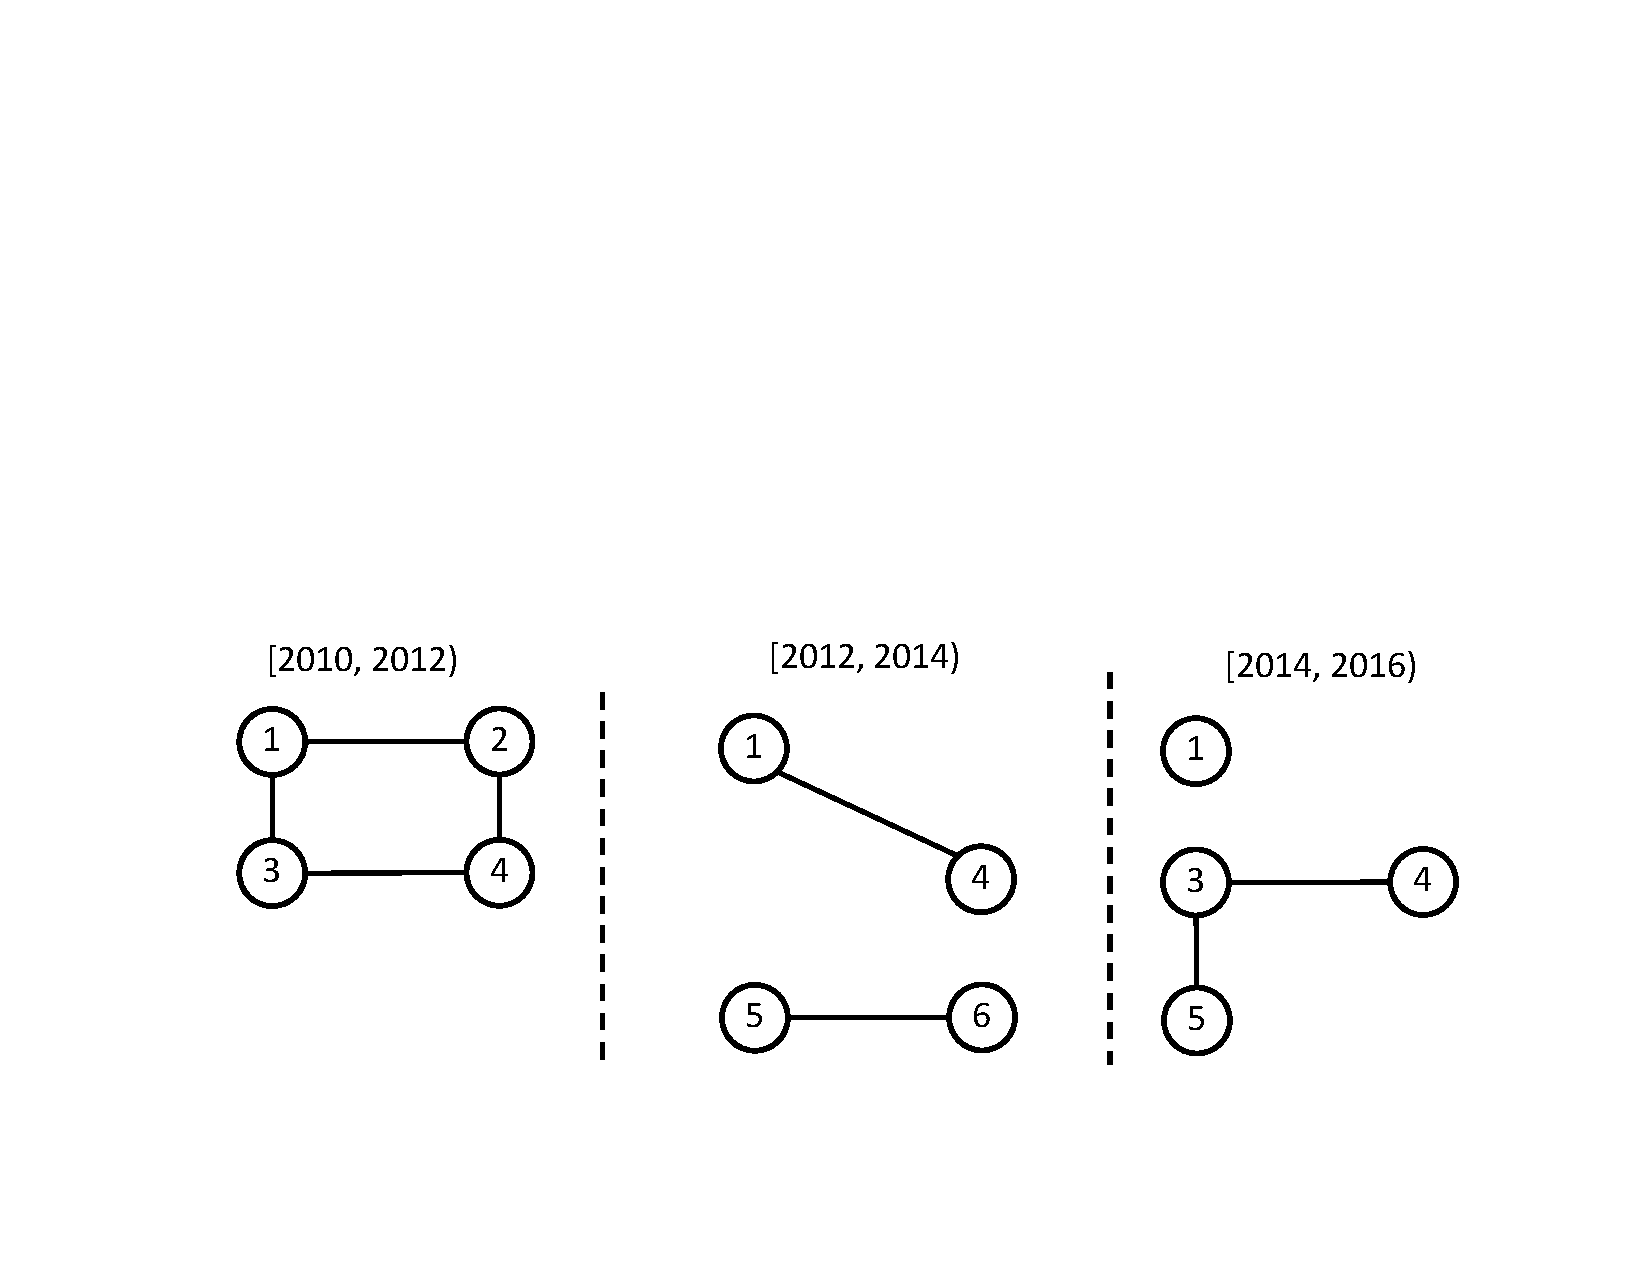
\includegraphics[width=3.2in]{figs/TGroupAll.pdf}
\caption{Result of query Q4.}
\label{fig:tg_all}
\end{figure}

Query Q4 illustrates another important feature of \ql, namely,
aggregation of values of non-key attributes of vertices and edges.  We
make the following operations available in \ql: \tt{min}, \tt{max},
\tt{sum}, \tt{count}, \tt{first}, \tt{last}, and \tt{any}.  To
illustrate, consider vertex and edge relations in
Figure~\ref{fig:rels} that correspond to the first two snapshots of
\tt{T}.  Vertex 1 is present in both $[2010, 2011)$ and $[2011,
    2012)$, and so also is present in the first snapshot of \tt{T3}.
    Vertex 1 has the same value for \tt{name} but different values for
    \tt{salary} in $[2010, 2011)$ and $[2011, 2012)$.  Therefore,
        taking any value of \tt{name} may be appropriate.  Returning
        to query Q3, when aggregation of attribute values is not
        specified explicitly, \tt{any} is used as the default for
        non-key attributes.  In the current version of \ql we require
        that $V$ and $E$ be grouped by their respective key
        attributes.  We may relax this restrictions in future versions
        of the system, to support structural aggregation of snapshots.
        Further, we require that values of all other attributes be
        aggregated with one of the provided operators.  We will
        provide additional operators in the future that return
        non-atomic data types like lists and maps, and will also allow
        developers to specify custom aggregation operators using our
        API.

\begin{verbatim}
  TSelect   Any V [vid, any(name), max(salary)] ; Any E [vid1, vid2, sum(cnt)]
  From      T
  TGroup    by 2 years
\end{verbatim}

\begin{verbatim}
  TSelect   Any V [id, any(name), max(salary), pagerank()]; Any E   
  From      T
  Start     2000 End  2004
  TAgg      by 2 years
\end{verbatim}

\begin{verbatim}
TSelect   Any V; Any E
From      T1 TOr T2
\end{verbatim}

\begin{verbatim}
  TSelect   Any V [id, any(name)]; Any E [id1, id2]
  From      T1 TAnd T2
  TGroup  by 2 years
\end{verbatim}

\begin{verbatim}
  TSelect   Any V [id, any(name)]; Any E [id1, id2]
  From      (TSelect All V [id, any(name); All E [id1, id2, any(name)]
             From T1 TAnd T2
            )
  TGroup  by 2 years
\end{verbatim}

\begin{verbatim}
  TSelect   All V[id, any(name), pagerank()]; All E[id1, id2, sum(cnt)]
  From      T1 TAnd  
           (TSelect   Any V; Any E
            From    T1 TAnd T2)
  TAgg    by 2 years
\end{verbatim}
